\newpage
%**************************************************************
\chapter{Il quadro strategico}
\label{cap:ilquadrostrategico}

\section{Strategie aziendali di stage}

L'azienda The White Dog s.r.l. accoglie e offre l'attività di stage per due principali motivi:

\begin{itemize}
	\item \textbf{Sperimentazione su progetti innovativi:} data la forte propensione alla ricerca dell'azienda, esistono numerosi campi che essa vorrebbe esplorare ma che a causa di altri progetti più prioritari e scarsità di tempo non può studiare. Offre quindi allo studente universitario un progetto di ricerca e sviluppo su tecnologie innovative ed interessanti, non pretendendo alcun risultato da subito inseribile nel mercato. Questo permette allo studente di vivere l'esperienza dello stage in piena libertà e serenità, riuscendo così a portare un notevole valore aggiunto personale che l'azienda è ben felice di accogliere;
	\item \textbf{Valutazione dello stagista:} l'azienda è in continua crescita e necessita di nuovo personale preparato e soprattutto capace di lavorare in costante sintonia col gruppo. Lo stage universitario permette all'azienda di scoprire persone che soddisfano questi due importanti requisiti per una futura assunzione.
\end{itemize}

Da parte sua The White Dog s.r.l. offre molto agli stagisti. I tutor aziendali supportano lo studente per tutto il periodo lavorativo, consigliandolo sia per quanto riguarda il piano di lavoro, sia sulle tecnologie da utilizzare sia effettuando proficue discussioni in vista della relazione finale. Allo studente viene offerto un ambiente di lavoro accogliente e strumenti aggiornati e all'avanguardia, supportandolo anche economicamente prevedendo un rimborso spese.

\section{Il progetto di stage proposto}

Il progetto propostomi nasce dalla costante volontà aziendale di ricercare nuove metodologie di interazione da proporre agli utenti dei suoi \textit{e-commerce} in ottica \textit{omni-channel}\ped{\hyperlink{oc}{G}}. Lo studio sulle nuove tecnologie e strumentazioni presenti sul mercato, ha portato l'azienda a considerare la realtà virtuale un terreno interessante e degno di studio. Nasce così l'idea di un \textit{e-commerce VR}, progetto in grado di colmare, in parte, quel divario che da sempre ha distanziato \textit{store} virtuale e negozio fisico.

\label{Omni-channel}
\begin{figure}[ht]
	\begin{center}
		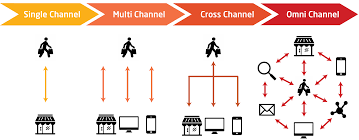
\includegraphics[scale=1]{omni-channel}
		\caption{Schema rappresentativo della differenze tra \textit{single-channel}, \textit{multi-channel}, \textit{cross-channel} e \textit{omni-channel}}
	\end{center}
\end{figure}
\FloatBarrier

L'obbiettivo di stage è, dunque, un'esplorazione tecnologica nel campo della \textit{vitual reality}\ped{\hyperlink{vr}{G}}. Il progetto, diviso in due parti, mira ad arrivare ad un prototipo di \textit{vitual showroom} dove poter esplorare ed interagire con i prodotti e permetterne l'acquisto. \\
La prima parte è relativa alla progettazione e realizzazione del movimento in uno spazio 3D ed interazione con gli oggetti. \\
La seconda parte tratta invece la progettazione e realizzazione in un'interfaccia di presentazione del prodotto, con integrazione al processo di acquisto mediante l'uso di sistemi \textit{cloud} esterni.

\subsection{Piano di lavoro proposto}

\subsubsection{Piano temporale}

In accordo col tutor aziendale, la durata massima dello stage è stata fissata a 320 ore, divise in 8 settimane lavorative di 5 giorni, 8 ore al giorno. \\
Il piano lavorativo è stato dunque pianificato nel seguente modo:

\begin{itemize}
	\item \textbf{Settimana 1:} analisi dei requisiti funzionali del sistema da sviluppare. Studio delle tecnologie e linguaggi disponibili riguardanti la realtà aumentata;
	
	\item \textbf{Settimana 2:} scelta dell'hardware da utilizzare in base ai requisiti. Scelta del \textit{framework}\ped{\hyperlink{fw}{G}} di sviluppo e primo prototipo di una scena 3D;
	
	\item \textbf{Settimana 3:} raffinamento della scena 3D, progettazione e sviluppo di oggetti e comportamento di essi nello spazio 3D. Primo prototipo di \textit{user interaction};
	
	\item \textbf{Settimana 4:} progettazione e sviluppo integrazione tra sistema \textit{VR}\ped{\hyperlink{vr}{G}} e \textit{e-commerce}. Progettazione di \textit{user interaction} per la fruizione dei contenuti provenienti dall'\textit{e-commerce};
	
	\item \textbf{Settimana 5:} approfondimento di \textit{user interaction} e del comportamento degli oggetti nell'ambiente virtuale;
	
	\item \textbf{Settimana 6:} studio e prototipazione del possibile processo d'acquisto all'interno dell'ambiente virtuale;
	
	\item \textbf{Settimana 7:} Conclusione del prototipo e della relativa documentazione;
	
	\item \textbf{Settimana 8:} studio del modello emergente di \textit{omni-channel}\ped{\hyperlink{oc}{G}} e come la realtà virtuale e la realtà aumentata possono estendere questo modello.
\end{itemize}

\subsubsection{Piano metodologico}
	
Assieme al tutor aziendale, abbiamo fin da subito concordato la mia presenza durante l'orario d'ufficio, permettendo così un interazione intensa e costante. \\
Il lavoro di ricerca e sviluppo che ho effettuato è stato totalmente autonomo, con giornaliere interazioni con il personale solo per raccogliere e analizzare la documentazione, requisiti e \textit{feedback} sull'andamento del progetto.
Le revisioni di progetto sono avvenute secondo la seguente metodologia:

\begin{itemize}
	\item Riunione breve di 15 minuti ogni mattina;
	\item Riunione di 1 ora alla fine di ogni settimana come analisi retrospettiva.
\end{itemize}  

\subsubsection{Piano tecnologico}

In questa sezione descriverò lo stack tecnologico inizialmente propostomi dall'azienda e di come si sia evoluto nel tempo dopo le attività di ricerca.

\subsection{Obiettivi aziendali}

In questa sottosezione elencherò gli obiettivi che l'azienda si pone di raggiungere con il mio stage.

\subsection{Obiettivi personali}

In questa sottosezione tratterò degli obbiettivi personali e delle motivazioni che mi hanno spinto a scegliere questo stage e questo progetto.



